\documentclass[11pt]{article}
\newcommand{\todo}[1]{{\color{red}[TODO: #1]}}

%%%%%%%%%%%%%%%%%%%%%%%%%%%%%%%%%%%%%%%%%%%%%%%%%%%%%%%%%%%%%%%%%
%%%%%%%%%%%%%%%%%%%%%%%%%%%%%%%%%%%%%%%%%%%%%%%%%%%%%%%%%%%%%%%%%
%%% PACKAGES
%%%%%%%%%%%%%%%%%%%%%%%%%%%%%%%%%%%%%%%%%%%%%%%%%%%%%%%%%%%%%%%%%
%%%%%%%%%%%%%%%%%%%%%%%%%%%%%%%%%%%%%%%%%%%%%%%%%%%%%%%%%%%%%%%%%
\usepackage[margin=2cm]{geometry}

\usepackage{amsmath} 
%\usepackage{amssymb} 
\usepackage{amsthm}

\usepackage{latexsym} % For \Box and \Diamond
\usepackage{colonequals} % for ::=
%\usepackage{bm} % nice boldface for maths

\usepackage[matrix,arrow]{xy}
%\usepackage{xcolor}
\usepackage[noxy]{virginialake}

%\usepackage{array}
\usepackage{graphicx} % For command \includegraphics and \scalebox                        
%\usepackage{tikz}

%\usepackage{lmodern} % Latin modern fonts in outline formats
%\usepackage{mathtools} % a se­ries of pack­ages de­signed to en­hance the ap­pear­ance of doc­u­ments con­tain­ing a lot of math­e­mat­ics
%\usepackage{enumerate} % adds an optional [style] argument to the enumerate environment

%\usepackage{pgf} % macro package for creating graphics
%\usepackage{pgffor}

%\usepackage{hyperref} % handle cross-referencing commands with hypertext links

%\usepackage{float} % for defining floating objects such as figures and tables
%\floatstyle{boxed} 
%\restylefloat{figure}

%%%%%%%%%%%%%%%%%%%%%%%%%%%%%%%%%%%%%%%%%%%%%%%%%%%%%%%%%%%%%%
%%%%%%%%%%%%%%%%%%%%%%%%%%%%%%%%%%%%%%%%%%%%%%%%%%%%%%%%%%%%%%
%%% Small equation environments
\newdimen\mydisplayskip
\mydisplayskip=.4\abovedisplayskip
%\newenvironment{smallequation}
%{\par\nobreak\vskip\mydisplayskip\noindent\bgroup\small\csname equation\endcsname}{\csname endequation\endcsname\egroup}
%%
\newenvironment{smallequation*}
{\par\nobreak\vskip\mydisplayskip\noindent\bgroup\small\csname equation*\endcsname}{\csname endequation*\endcsname\egroup}
%%
%\newenvironment{smallalign}
%{\par\nobreak\noindent\bgroup\small\csname align\endcsname}{\csname endalign\endcsname\egroup}
%%
%\newenvironment{smallalign*}
%{\par\nobreak\noindent\bgroup\small\csname align*\endcsname}{\csname endalign*\endcsname\egroup}

%%%%%%%%%%%%%%%%%%%%%%%%%%%%%%%%%%%%%%%%%%%%%%%%%%%%%%%%%%%%%%
%%%%%%%%%%%%%%%%%%%%%%%%%%%%%%%%%%%%%%%%%%%%%%%%%%%%%%%%%%%%%%
%%%% Theorem counter
\theoremstyle{plain}
\newtheorem{theorem}{Theorem}[section]
%\newtheorem{conjecture}[theorem]{Conjecture}
%\newtheorem{fact}[theorem]{Fact}
%\newtheorem{claim}[theorem]{Claim}
\newtheorem{proposition}[theorem]{Proposition}
\newtheorem{lemma}[theorem]{Lemma}
%\newtheorem{corollary}[theorem]{Corollary}
%%
\theoremstyle{definition}
%\newtheorem{observation}[theorem]{Observation}
\newtheorem{definition}[theorem]{Definition}
%\newtheorem{problem}[theorem]{Problem}
%\newtheorem{construction}[theorem]{Construction}
\newtheorem{remark}[theorem]{Remark}

%%%%%%%%%%%%%%%%%%%%%%%%%%%%%%%%%%%%%%%%%%%%%%%%%%%%%%%%%%%%%%%%%
%%%%%%%%%%%%%%%%%%%%%%%%%%%%%%%%%%%%%%%%%%%%%%%%%%%%%%%%%%%%%%%%%
%%%% 
%\tikzset{
%	annotated cuboid/.pic={
%		\tikzset{%
%			every edge quotes/.append style={midway, auto},
%			/cuboid/.cd,
%			#1
%		}
%		\draw [every edge/.append style={pic actions, opacity=.5}, pic actions]
%		(0,0,0) coordinate (o) -- ++(-\cubescale*\cubex,0,0) coordinate (a) -- ++(0,-\cubescale*\cubey,0) coordinate (b) edge coordinate [pos=1] (g) ++(0,0,-\cubescale*\cubez)  -- ++(\cubescale*\cubex,0,0) coordinate (c) -- cycle
%		(o) -- ++(0,0,-\cubescale*\cubez) coordinate (d) -- ++(0,-\cubescale*\cubey,0) coordinate (e) edge (g) -- (c) -- cycle
%		(o) -- (a) -- ++(0,0,-\cubescale*\cubez) coordinate (f) edge (g) -- (d) -- cycle;
%		
%		;
%	},
%	/cuboid/.search also={/tikz},
%	/cuboid/.cd,
%	width/.store in=\cubex,
%	height/.store in=\cubey,
%	depth/.store in=\cubez,
%	units/.store in=\cubeunits,
%	scale/.store in=\cubescale,
%	width=10,
%	height=10,
%	depth=10,
%	units=cm,
%	scale=.1,
%}
%%tikz parameters
%
%\tikzstyle{point}=[circle,draw]
%\usetikzlibrary{arrows,automata,shapes,decorations.markings,
%	decorations.pathmorphing,backgrounds,fit,snakes,calc}
%

%%%%%%%%%%%%%%%%%%%%%%%%%%%%%%%%%%%%%%%%%%%%%%%%%%%%%%%%%%%%%%%%%
%%%%%%%%%%%%%%%%%%%%%%%%%%%%%%%%%%%%%%%%%%%%%%%%%%%%%%%%%%%%%%%%%
%%%% Extracting symbols from MnSymbol 
\DeclareFontFamily{U} {MnSymbolC}{}
%
\DeclareFontShape{U}{MnSymbolC}{m}{n}{
	<-6>  MnSymbolC5
	<6-7>  MnSymbolC6
	<7-8>  MnSymbolC7
	<8-9>  MnSymbolC8
	<9-10> MnSymbolC9
	<10-12> MnSymbolC10
	<12->   MnSymbolC12}{}
\DeclareFontShape{U}{MnSymbolC}{b}{n}{
	<-6>  MnSymbolC-Bold5
	<6-7>  MnSymbolC-Bold6
	<7-8>  MnSymbolC-Bold7
	<8-9>  MnSymbolC-Bold8
	<9-10> MnSymbolC-Bold9
	<10-12> MnSymbolC-Bold10
	<12->   MnSymbolC-Bold12}{}
%
\DeclareSymbolFont{MnSyC}         {U}  {MnSymbolC}{m}{n}
%
\DeclareMathSymbol{\diamondplus}{\mathbin}{MnSyC}{124}
\DeclareMathSymbol{\boxtimes}{\mathbin}{MnSyC}{117}


%%%%%%%%%%%%%%%%%%%%%%%%%%%%%%%%%%%%%%%%%%%%%%%%%%%%%%%%%%%%%%%%%
%%%%%%%%%%%%%%%%%%%%%%%%%%%%%%%%%%%%%%%%%%%%%%%%%%%%%%%%%%%%%%%%%
%%%% Virginialake add-ons
\newcommand{\vlderivationauxnc}[1]{#1{\box\derboxone}\vlderivationterm}
\newcommand{\vlderivationnc}{\vlderivationinit\vlderivationauxnc}
%
%
\makeatletter
\newbox\@conclbox
\newdimen\@conclheight
%
%
\newcommand{\vlhtr}[2]{\vlpd{#1}{}{#2}}
\newcommand\vlderiibase[5]{{%
		\setbox\@conclbox=\hbox{$#3$}\relax%
		\@conclheight=\ht\@conclbox%
		\setbox\@conclbox=\hbox{$%
			\vlderivationnc{%
				\vliin{#1}{#2}{\box\@conclbox}{#4}{#5}%
			}$}%
		\lower\@conclheight\box\@conclbox%
	}}
	%
	\newcommand\vlderibase[4]{{%
			\setbox\@conclbox=\hbox{$#3$}\relax%
			\@conclheight=\ht\@conclbox%
			\setbox\@conclbox=\hbox{$%
				\vlderivationnc{%
					\vlin{#1}{#2}{\box\@conclbox}{#4}%
				}$}%
			\lower\@conclheight\box\@conclbox%
		}}
		%
		\newcommand\vlderidbase[4]{{%
				\setbox\@conclbox=\hbox{$#3$}\relax%
				\@conclheight=\ht\@conclbox%
				\setbox\@conclbox=\hbox{$%
					\vlderivationnc{%
						\vlid{#1}{#2}{\box\@conclbox}{#4}%
					}$}%
				\lower\@conclheight\box\@conclbox%
			}}
			%
			\makeatother
			%


%%%%%%%%%%%%%%%%%%%%%%%%%%%%%%%%%%%%%%%%%%%%%%%%%%%%%%%%%%%%%%%%%
%%%%%%%%%%%%%%%%%%%%%%%%%%%%%%%%%%%%%%%%%%%%%%%%%%%%%%%%%%%%%%%%%
%%% MACROS
%%%%%%%%%%%%%%%%%%%%%%%%%%%%%%%%%%%%%%%%%%%%%%%%%%%%%%%%%%%%%%%%%
%%%%%%%%%%%%%%%%%%%%%%%%%%%%%%%%%%%%%%%%%%%%%%%%%%%%%%%%%%%%%%%%%

%%%% Comments  
\definecolor{notgreen}{rgb}{.1,.6,.1}
\newcommand{\marianela}[1]{{\color{purple}[Marianela: #1]}}
\newcommand{\sonia}[1]{{\color{blue}[Sonia: #1]}}
\newcommand{\lutz}[1]{{\color{notgreen}[Lutz: #1]}}
%\newcommand{\todo}[1]{{\color{red}[TODO: #1]}}

%%%% General
\newcommand*{\A}{\mathcal{A}}
%\newcommand{\G}{\mathcal{G}}
\newcommand*{\SG}{\fm{\mathcal{G}}}
\newcommand{\SGi}[1]{\fm{\mathcal{G}_{#1}}}
%
\newcommand{\quand}{\quad\mbox{and}\quad}
\newcommand{\qquand}{\qquad\mbox{and}\qquad}
\newcommand{\quadcm}{\rlap{\quad,}}
%
\newcommand{\proviso}[1]{\mbox{\scriptsize #1}}

%%%% Systems
\newcommand*{\ax}[1]{\mathsf{#1}}
\newcommand*{\kax}[1][]{\ax{k_{#1}}}
\newcommand{\fourax}{\ax{4}}
\newcommand{\agklmn}{\mathsf{g_{klmn}}}
%
\newcommand*{\IK}{\mathsf{IK}}
\newcommand*{\K}{\mathsf{K}}
%
\newcommand*{\IKfour}{\mathsf{IK4}}
\newcommand*{\Kfour}{\mathsf{K4}}
%
%\newcommand*{\ISfour}{\mathsf{IS4}}
%\newcommand*{\Sfour}{\mathsf{S4}}
%
\newcommand*{\labIKp}{\lab\IK_{\le}}

%%%% Connectives
\newcommand*{\NOT}{\neg}
\newcommand*{\AND}{\mathbin{\wedge}}
\newcommand*{\TOP}{\mathord{\top}}
\newcommand*{\OR}{\mathbin{\vee}}
\newcommand*{\BOT}{\mathord{\bot}}
\newcommand*{\IMP}{\mathbin{\supset}}%%\scalebox{.9}{\raise.2ex\hbox{$\supset$}}}}

\newcommand*{\BOX}{\mathord{\Box}}
\newcommand*{\DIA}{\mathord{\Diamond}}
%
%%%% Labelled sequents
\newcommand{\lseq}[3]{#1 , #2 \SEQ #3}
%
\newcommand{\B}{\mathcal{R}}
\newcommand{\Left}{\Gamma} %{\mathcal{L}}
\newcommand{\Right}{\Delta} %{\mathcal{R}}
%
\newcommand*{\fm}[1]{{\color{notgreen}{#1}}}
\newcommand*{\lb}[1]{{\color{blue}{#1}}}
%
\newcommand*{\rel}{R}
\newcommand*{\labels}[2]{\lb{#1}\mathord{:}\fm{#2}}
\newcommand*{\accs}[2]{\lb{#1}R\lb{#2}}
\newcommand*{\futs}[2]{\lb{#1}\le{\lb{#2}}}
%
\newcommand{\SEQ}{\Longrightarrow}
%

%%%% Labelled rules
\newcommand*{\rn}[1]  {\ensuremath{\mathsf{#1}}}
\newcommand*{\lab}{\mathsf{lab}}
%
\newcommand*{\labrn}[2][]  {\rn{#2}_{#1}}%^{\lab}}}
\newcommand*{\rlabrn}[2][]  {\rn{#2}_\rn{R#1}}%^\lab}}
\newcommand*{\llabrn}[2][]  {\rn{#2}_\rn{L#1}}%^\lab}}
%%
%\newcommand*{\brsym}{\boxtimes}%\mathord{\scalebox{.8}{$\blacksquare$}}}
\newcommand*{\diasym}{\diamondplus}%\mathord{\blacklozenge}}
%%
\newcommand*{\boxbrn}[1]{\boxtimes_\rn{#1}}%^{\lab}}}
\newcommand*{\diabrn}[1]{\diamondplus_\rn{#1}}

%%%% System labIK+gklmn
\newcommand{\gklmn}{\boxtimes_{\mathsf{gklmn}}}
\newcommand{\boxk}{\square_{R}^{k}}
\newcommand{\boxlk}{\square_{L}^{k}}
\newcommand{\diamk}{\lozenge_{L}^{k}}
\newcommand{\diamrk}{\lozenge_{R}^{k}}

%%%% Semantics
\newcommand{\f}{f^{\mathcal{M}}}
\newcommand{\M}{\mathcal{M}}
\newcommand{\F}{\mathcal{F}}
%
\newcommand{\inter}[1]{\lb{\llbracket #1\rrbracket}}
%\newcommand{\force}[3]{#1,#2\Vdash#3}
\newcommand{\nforce}[3]{#1,#2\not\Vdash#3}
\newcommand{\cforce}[3]{#1,\lb{#2}\Vdash\fm{#3}}
\newcommand{\cnforce}[3]{#1,\lb{#2}\not\Vdash\fm{#3}}

%%%% Derivations
\newcommand{\Dw}{\mathcal{D}^{\rn w}}
\newcommand{\Dwone}{\mathcal{D}_{1}^{\rn w}}
\newcommand{\Dwtwo}{\mathcal{D}_{2}^{\rn w}}
%
\newcommand{\D}{\mathcal{D}}
\newcommand*{\DD}{\mathcal{D}}
\newcommand{\Done}{\mathcal{D}_{1}}
\newcommand{\Dtwo}{\mathcal{D}_{2}}
%
\newcommand{\height}[1]{|#1|}
%
\newcommand*{\reducesto}{\quad{\leadsto}\quad}
\newcommand*{\invr}[1]{#1}%^\bullet}



%%Symbols for System labK
%\newcommand{\id}{id^{lab}}
%\newcommand{\tolab}{\top^{lab}}
%\newcommand{\vlab}{\wedge^{lab}}
%\newcommand{\olab}{\vlor^{lab}}
%\newcommand{\blab}{\square^{lab}}
%\newcommand{\dlab}{\lozenge^{lab}}
%
%%Labelled proof system
%\newcommand{\toprule}{\B \Rightarrow \Right, x  \colon   \top}
%\newcommand{\vlabr}{\B \Rightarrow \Right, x  \colon   A}
%\newcommand{\vlabu}{\B \Rightarrow \Right, x  \colon   B}
%\newcommand{\olabr}{\B \Rightarrow \Right, x  \colon   A, x  \colon   B}
%\newcommand{\blabr}{\B \Rightarrow \Right, x  \colon   \square A}
%\newcommand{\blabu}{\B, x$R$y \Rightarrow \Right, y  \colon   A}
%\newcommand{\dlabr}{\B, x$R$y \Rightarrow \Right, x  \colon   \lozenge A}
%\newcommand{\dlabu}{\B, x$R$y \Rightarrow \Right, x  \colon   \lozenge A, y  \colon} 
%
%
%%Symbols for system labIK
%\newcommand{\botlab}{\bot_{L}^{lab}}
%\newcommand{\toplab}{\top_{R}^{lab}}
%\newcommand{\andleflab}{\wedge_{L}^{lab}}
%\newcommand{\andriglab}{\wedge_{R}^{lab}}
%\newcommand{\orleflab}{\vlor_{L}^{lab}}
%\newcommand{\orriglabo}{\vlor_{R1}^{lab}}
%\newcommand{\orriglabt}{\vlor_{R2}^{lab}}
%\newcommand{\irlab}{\vljm_{R}^{lab}}
%\newcommand{\illab}{\vljm_{L}^{lab}}
%\newcommand{\dllab}{\lozenge_{L}^{lab}}
%\newcommand{\drlab}{\lozenge_{R}^{lab}}
%\newcommand{\bllab}{\square_{L}^{lab}}
%\newcommand{\brlab}{\square_{R}^{lab}}
%
%%Symbols for System labheartIK
%\newcommand{\ids}{id}
%\newcommand{\idg}{id_{g}}
%\newcommand{\refl}{refl}
%\newcommand{\trans}{trans}
%\newcommand{\cut}{cut}
%\newcommand{\fone}{F1}
%\newcommand{\ftwo}{F2}
%\newcommand{\sbot}{\bot_{L}}
%\newcommand{\Stop}{\top_{R}}
%\newcommand{\svlef}{\wedge_{L}}
%\newcommand{\svrig}{\wedge_{R}}
%\newcommand{\solef}{\vlor_{L}}
%\newcommand{\sorig}{\vlor_{R}}
%\newcommand{\sorone}{\vlor_{R1}}
%\newcommand{\sotwo}{\vlor_{R2}}
%\newcommand{\sir}{\vljm_{R}}
%\newcommand{\sil}{\vljm_{L}}
%\newcommand{\sdl}{\lozenge_{L}}
%\newcommand{\sdr}{\lozenge_{R}}
%\newcommand{\sbl}{\square_{L}}
%\newcommand{\sbr}{\square_{R}}
%\newcommand{\smon}{mon_{L}}
%%
%\newcommand{\Gone}{\mathcal{G}_{1}}
%\newcommand{\Gtwo}{\mathcal{G}_{2}}
%
%% System LABIK
%\newcommand{\conjrig}{\G, \Left \Rightarrow \Right, x \colon A}
%\newcommand{\conjrigh}{\G, \Left \Rightarrow \Right, x  \colon B}
%\newcommand{\conjlef}{\G, \Left, x  \colon  A, x \colon B \Rightarrow \Right}


\begin{document}


\textbf{Review 1}

\begin{itemize}
	\item \emph{Also the proofs of the structural properties closely follow the methodology of the paper by Maffezioli, Naibo \& Negri. All this has to be said expressis verbis, and appropriate citations have to be added.
	Perhaps even more importantly, the authors of the paper under review neglect an important caveat in the design of rules of contraction-free labelled sequent calculi: to guarantee that contraction be admissible one needs to ensure that a certain closure condition be satisfied, see:}
	
		\emph{• Negri, S. Proof analysis in modal logic. Journal of Philosophical Logic, 34, 507–544, 2005.}
		\begin{center}
			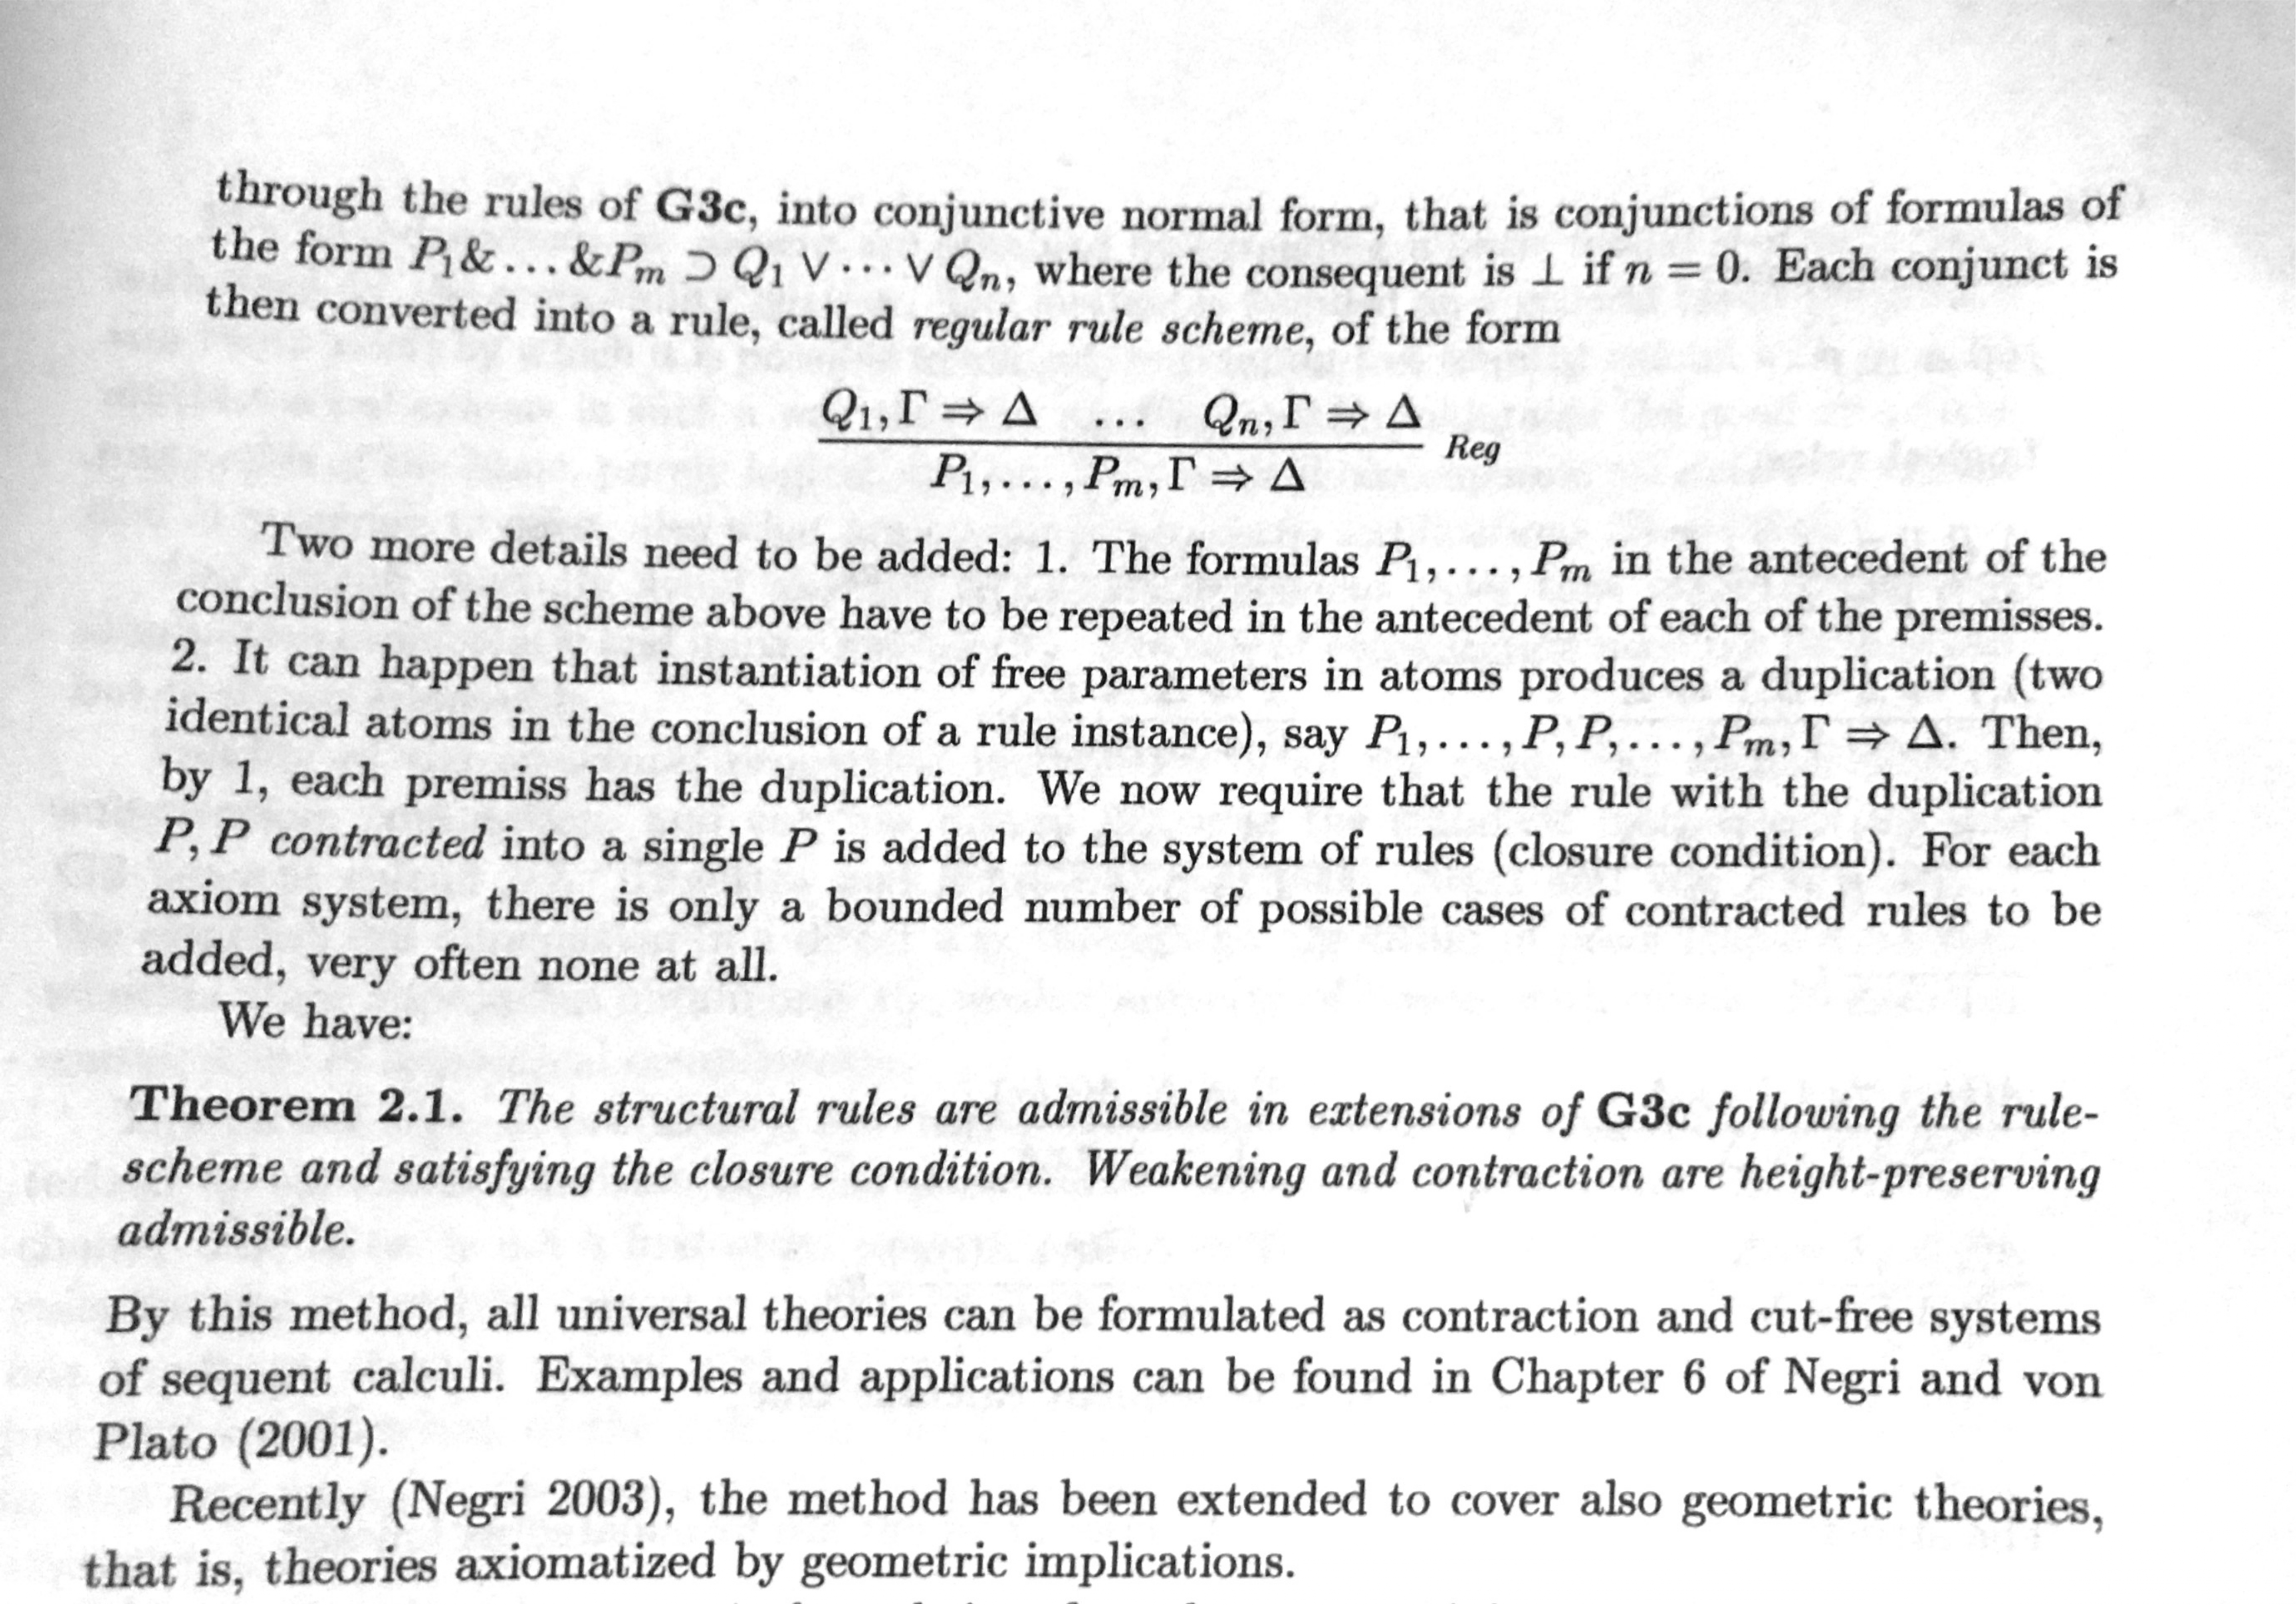
\includegraphics[scale=.18]{closure-condition-Negri}
		\end{center}
	
\end{itemize}
\todo{Add next remark to the paper} 

\begin{remark}
	
	The rules $\llabrn{cont}$ and $\rlabrn{cont}$ are admissible for $\labIKp$.
	\begin{center}
		$\vlinf{\llabrn{cont}}{}{\B, \Left, \labels{x}{A} \SEQ \Right}{\B, \Left, \labels{x}{A}, \labels{x}{A} \SEQ \Right}$\quad\quad$\vlinf{\rlabrn{cont}}{}{\B, \Left \SEQ \Right, \labels{x}{A}}{\B, \Left \SEQ \Right, \labels{x}{A}, \labels{x}{A}}$
	\end{center}
\end{remark}
\begin{proof}
	The rule $\llabrn{cont}$ can be derived using $\rn{refl}$ and $\llabrn{mon}$ which is admissible by Proposition 3.1.
	
	\begin{center}
			$\vlderivation{
				\vlin{\rn{refl}}{}
				{\B, \Left, \labels{x}{A} \SEQ \Right}
				{\vlin{\llabrn{mon}}{}
					{\B, \futs{x}{x}, \Left, \labels{x}{A} \SEQ \Right}
					{\vlhy{\B, \futs{x}{x}, \Left, \labels{x}{A}, \labels{x}{A} \SEQ \Right}}}
			}$
	\end{center}

The case for $\rlabrn{cont}$ is similar.
\end{proof}

\begin{itemize}
	\item \emph{In Section 7, if the rules G klmn are added without their contracted instances, the calculus will not be complete. For example, in the classical case, Euclidean transitivity $\forall a,b,c (\accs{a}{b} \& \accs{a}{c} \IMP \accs{b}{c})$ has the contracted instance $\forall a,b (\accs{a}{b} \IMP \accs{b}{b})$ that allows for the derivation of $ \BOX(\BOX A \IMP A)$. This, however, can hardly be derived without the rule’s contracted instance.}
\end{itemize}

\todo{Add next proof as an example} \marianela{How should I introduce this in the extensions section?}
$$
	\vlderivation{
		\vlin{\rlabrn\BOX}{}{\SEQ \labels{x}{\BOX(\BOX A \IMP A)}}{
			\vlin{\rlabrn\IMP}{\lb v\mbox{ fresh}}{\futs xy, \accs yz \SEQ \labels{z}{\BOX A \IMP A}}{
				\vlin{\rn F_1}{\lb u\mbox{ fresh}}{\futs xy, \accs yz, \futs zv, \labels{v}{\BOX A} \SEQ \labels{v}{A}}{
					\vlin{\rn g_{1110}}{ \lb{w}\mbox{ fresh}}{\futs xy, \accs yz, \futs zv, \futs yu, \accs uv, \labels{v}{\BOX A} \SEQ \labels{v}{A}}{
							\vlin{\llabrn\BOX}{}{\futs xy, \accs yz, \futs zv, \futs yu, \accs uv, \futs{v}{w}, \accs{w}{v}, \labels{v}{\BOX A} \SEQ \labels{v}{A}}{
								\vlin{\rn{id}}{}{\futs xy, \accs yz, \futs zv, \futs yu, \accs uv, \futs{v}{w}, \accs{w}{v}, \labels{v}{\BOX A}, \labels{v}{A} \SEQ \labels{v}{A}}{
									\vlhy{}
							}
						}
					}
				}
			}
		}
	}
$$

\begin{itemize}
	\item \emph{Also the reason for preferring one semantics for intuitionistic modal logic over another should be discussed in
	detail, as otherwise the authors’ work would rather look a routine exercise.}: \todo{add a paragraph about constructive modal logics.} \marianela{using the Skolemization thing (Review 2)?} 
	\item \todo{Add a paragraph with all the references we are missing.} 
	\item \emph{They then claim that their calculus is inspired by a ”multiple-conlusion nested sequent
		system a la Maehara”. Such a calculus in fact has appeared in a work which the authors	cite as unpublished, but which seems to have been published in the meantime [Archive for Mathematical Logic (2019) 58:359–385], which reference needs to be updated accordingly.} \marianela{What did she mean?}
	\item \emph{The rules of their calculus are identical (except for the ones that relate the two accessibility relations) to the rules for the intuitionistic-alethic fragment of the calculus for intuitionistic bimodal logic in this publication:
		• Maffezioli, P., Naibo, A. \& Negri, S., The Church-Fitch knowability paradox in the light of structural proof theory. Synthese, vol. 190, 2677–2716, 2013.} {\color{green}Fixed: adding that we have internal cut.}
\end{itemize}


\textbf{Review 2: TODO list}

\begin{itemize}
	\item \emph{Broken references “??” in pages 13 and 14}: {\color{green}Fixed.}
	\item \emph{The section of ``Extensions" has to be more detailed:
		\begin{itemize}
			\item it does not help at all that the
			applications of the rule g1111 are merged with $\llabrn\BOX$ and $\rlabrn\DIA$ in the example
			derivation. {\color{green}Fixed.}
			\item Most importantly, I am not convinced by the gklmn rule. The side condition stipulates that $\lb y'$ and $\lb u$ are fresh, whereas the frame property contains existential quantifications. I was thus expecting either a Skolemization in the style of Vigano in the ``Labelled Non-Classical Logics" book, or a geometric rule with existential quantification in the style of Simpson [Sim94] or, perhaps even better, a “mixed” rule where the labels are	assumed more or less in the style of an $\exists$ elimination to derive a labeled formula. \todo{SONIA}
		\end{itemize}}
	\item \emph{Remark 4.2. Show the ``need" you would likely have to show that no other proofs of the axioms are possible. That is of course the case, but unless you prove it formally, it is not fully correct to claim that the ``need'' is shown.} {\color{green}Fixed.}
	
	
	\item \todo{LUTZ: \emph{Reconsider de abstract. It reads very “operational” and does not clearly state the contributions of the paper.}}
\end{itemize}

We do not need contraction. We have an internal cut elimination. That's why it is a novelty.
\end{document}